\subsubsection{Server - OrderGateway}
\begin{figure}[H]
	\centering
	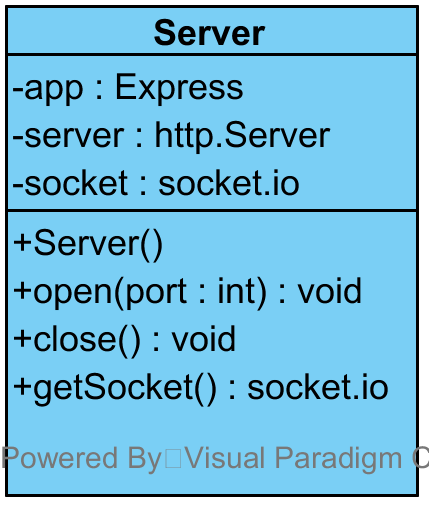
\includegraphics[width=15cm]{./diagrammi/demo/server.png}
	\caption{Componente OrderGateway}
\end{figure}
Il server è composto dall'OrderGateway, che ne è la base, dal package Order, che contiene le classi che rappresentano degli ordini, e da Menu, il quale 

\setclass{OrderGateway::Order}
\paragraph[::Order]{\class}\mbox{}\\ \label{\class}
\begin{figure}[H]
	\centering
	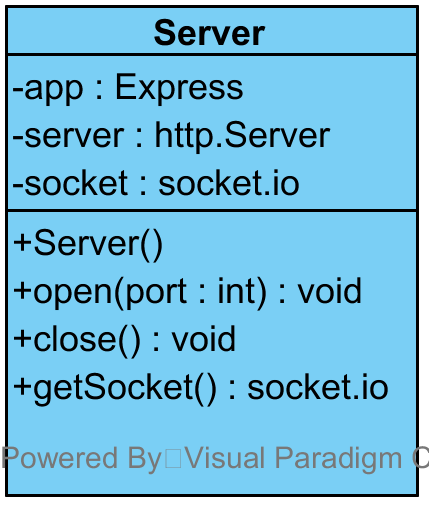
\includegraphics[width=15cm]{./diagrammi/demo/server.png}
	\caption{Componente OrderGateway}
\end{figure}

\setclass{OrderGateway::Order::Order}
\paragraph[::Order]{\class}\mbox{}\\ \label{\class}
\begin{figure}[H]
	\centering
	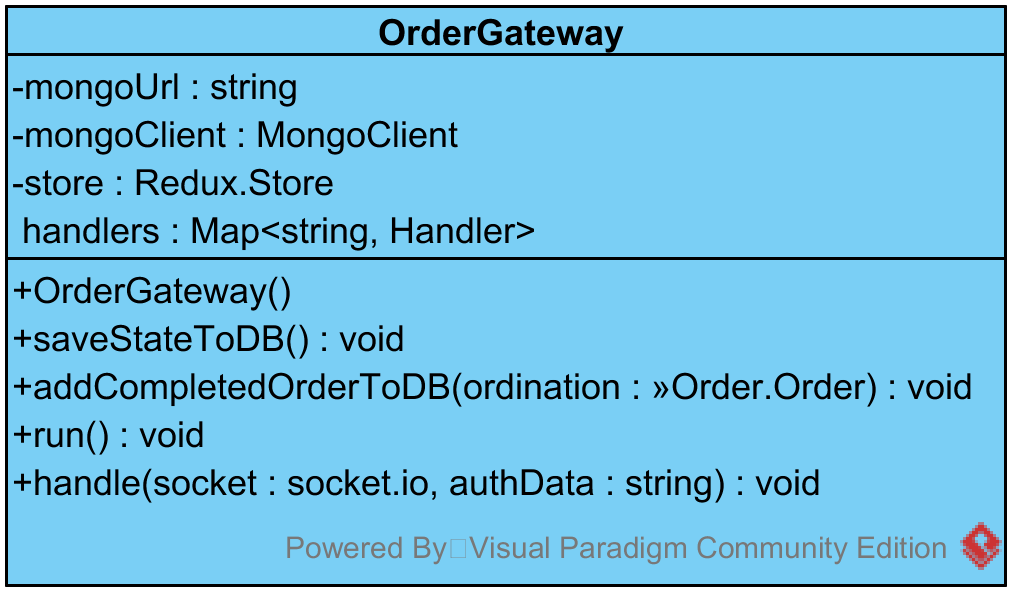
\includegraphics[width=15cm]{./diagrammi/demo/server/ordergateway.png}
	\caption{Classe \class}
\end{figure}
\textbf{Descrizione:}\\
Classe che inizializza le connessioni e prepara l'ambiente del server.

\textbf{Utilizzo:}\\
È la base del server e viene utilizzata per le 

\textbf{Classi ereditate:}
\begin{itemize}
	\item \code{EventEmitter}.
\end{itemize}

\textbf{Sottoclassi:}
\begin{itemize}
	\item \coderef{Framework::Model::API::ExternalAPI::ExternalAPIStore}.
\end{itemize}

%\textbf{Attributi:}
%
%\textbf{Metodi:}